\documentclass[conference]{IEEEtran}  % Use IEEE conference format

% Packages for math and symbols
\usepackage{amsmath, amssymb, amsthm}
\usepackage{mathpazo}      % Palatino font for a softer look
\usepackage{microtype}     % Better typography
\usepackage[T1]{fontenc}
\usepackage[utf8]{inputenc}
\usepackage{mathtools}     % Extension of amsmath with improvements
\usepackage{breqn}         % For breaking long equations automatically
\usepackage{bm}            % For bold math symbols

% Make equations respect column width
\allowdisplaybreaks
\setlength{\mathindent}{0pt}

% Hyperlinks and references
\usepackage{hyperref}
\hypersetup{
    colorlinks=true,
    linkcolor=blue,
    citecolor=blue,
    urlcolor=blue
}

% Title information
\title{\textbf{EUCLID: Multi-Head Binary Classification System for Synthetic Data Detection and Audio Authentication}}
\author{
    \IEEEauthorblockN{Sabian Hibbs BSc, MSc}
    \IEEEauthorblockA{Chief Technology Officer\\
    Uhmbrella Ltd.\\
    Email: sabian@uhmbrella.io}
}
\date{12/03/2025}

\begin{document}

\maketitle

\begin{abstract}
The proliferation of synthetically generated content presents a formidable challenge within contemporary machine learning paradigms, particularly in the domain of artificially generated audio. This white paper describes EUCLID (Enhanced Utility for Classification and Identification of Data), an innovative multi-head binary classification architecture that distinguishes between authentic and synthetic data through an ensemble of specialised neural network substructures. The proposed framework integrates sophisticated probabilistic formulations, a novel asymmetric output aggregation method, and a meticulously engineered data processing pipeline. This manuscript explains the theoretical foundations of the EUCLID model, using mathematical detail that clearly explains each computational module, and concludes with performance projections and future research directions.
\end{abstract}

\section{Introduction}
Detecting synthetic data, especially artificial audio, is a significant challenge in modern machine learning. This manuscript introduces a multi-head binary classification architecture designed to discriminate between authentic and synthetically generated data specimens. The framework integrates multiple neural network substructures (``heads''), whose outputs undergo a specialised aggregation protocol engineered to enhance detection sensitivity. This sophisticated approach incorporates a rigorous probabilistic formalism, an ensemble classification methodology with a novel asymmetric output-integration strategy, and a comprehensive data transformation pipeline. The system's modular design, encompassing all operational stages from preprocessing to inference, facilitates adaptability and renders it suitable for inclusion in technical documentation or project repositories.

The organisation of this discourse proceeds as follows: We commence with a formal mathematical exposition of the classification model, elucidating the probabilistic computation framework, loss function formulation, decision boundary determination methodology, and the theoretical justification for the distinctive averaging of ``authentic'' logits across multiple neural substructures. Subsequently, we provide exhaustive explications of each computational module within the implementation pipeline, articulating how the constituent scripts collectively form an integrated detection system:
\begin{itemize}
    \item \texttt{file\_renamer.py} -- ensures consistent, unique filenames for audio data.
    \item \texttt{audio\_converter.py} -- normalises audio format and sampling.
    \item \texttt{audio\_augment.py} -- generates augmented audio examples to expand the training set.
    \item \texttt{audio\_segmenter.py} -- chops audio files into fixed-length segments.
    \item \texttt{dataset\_manager.py} -- splits data into training and testing sets by class.
    \item \texttt{file\_manager.py} -- checks and fixes any overlap between training and testing sets (to prevent data leakage).
    \item \texttt{submodel\_trainer.py} -- trains individual classification sub-models (the ``heads'').
    \item \texttt{model\_merger.py} -- merges multiple trained sub-models into a unified multi-head ensemble model.
    \item \texttt{inference\_runner.py} -- runs the merged model on new data for inference, producing detection results.
\end{itemize}

Finally, we examine the performance characteristics of our multi-head classification architecture. The analysis includes projected accuracy metrics and computational efficiency assessments for the system's ensemble-based design and modular processing pipeline. We highlight how the combination of specialised detection heads contributes to overall system robustness and sensitivity in distinguishing between authentic and synthetic audio specimens.

\section{Multi-Head Classification Model: Mathematical Framework}
The core of the system is a binary classifier implemented as an ensemble of neural network sub-models (multiple ``heads''). Each sub-model is a deep neural network that independently attempts to classify an audio sample as Real (authentic) or Synthetic (fake). By combining several sub-models, the system aims to improve robustness and detection accuracy through ensemble learning. In this section, we detail the model architecture and derive its probability estimates, loss function formulation, decision strategy, and explain the reasoning for the unique averaging of real logits.

\subsection{Model Architecture and Probability Computation}
Each sub-model instantiates a convolutional neural architecture that operates on spectro-temporal representations of acoustic signals. In our implementation, individual sub-models utilise a \emph{pretrained convolutional backbone} (specifically, a residual network architecture such as ResNet-18) for extracting hierarchical feature representations from input spectrograms, followed by a domain-specific classification module that projects these representations onto a binary decision space. Formally, given an input representation \(x\) (a log-mel spectrogram derived from an audio segment), each sub-model \(f_i\) (parameterised by \(\theta_i\)) computes a two-dimensional projection into logit space:
\begin{equation}
\label{eq:submodel_output}
z_i = f_i(x; \theta_i) = \bigl(z_{i,\text{real}}, \; z_{i,\text{synthetic}}\bigr),
\end{equation}
where \(z_{i,\text{real}}\) is the logit (unnormalised score) that the sample is real, and \(z_{i,\text{synthetic}}\) is the logit that the sample is synthetic. (Some implementations may swap the order; what matters is consistent interpretation of each index.)

To convert logits into class probabilities for a given sub-model, we apply the softmax function. For sub-model \(i\), the predicted probability of the sample being real or synthetic is:
\begin{equation}
\label{eq:submodel_prob_real}
p_{i,\text{real}} = \frac{e^{z_{i,\text{real}}}}{e^{z_{i,\text{real}}} + e^{z_{i,\text{synthetic}}}},
\end{equation}
\begin{equation}
\label{eq:submodel_prob_synthetic}
p_{i,\text{synthetic}} = \frac{e^{z_{i,\text{synthetic}}}}{e^{z_{i,\text{real}}} + e^{z_{i,\text{synthetic}}}},
\end{equation}
which ensures \(p_{i,\text{real}} + p_{i,\text{synthetic}} = 1\). This is a special case of the softmax for \(C=2\) classes (binary classification), where we normalise the two logits to obtain a valid probability distribution. In general, for a classifier with \(C\) classes and logits \(z = (z_1, z_2, \dots, z_C)\), the softmax defines
\begin{equation}
\label{eq:softmax_general}
p_i = \frac{e^{z_i}}{\sum_{j=1}^{C} e^{z_j}}.
\end{equation}
Here \(C=2\), and it simplifies as above.

Our system combines \(N\) such sub-models. We construct a multi-head ensemble model \(F(x)\) that aggregates the outputs of all sub-models. The ensemble’s forward pass collates the logits from each sub-model:
\begin{itemize}
    \item For each sub-model \(i = 1, \dots, N\), compute \(z_i = (z_{i,\text{real}}, z_{i,\text{synthetic}})\).
    \item Separate the real and synthetic components: collect all \(z_{i,\text{real}}\) into a set \(\{z_{1,\text{real}}, \ldots, z_{N,\text{real}}\}\) and all synthetic logits \(\{z_{1,\text{synthetic}}, \ldots, z_{N,\text{synthetic}}\}\).
    \item The ensemble real logit is defined as the average of all real logits:
    \begin{equation}
    \label{eq:ensemble_real_logit}
    z_{\text{ensemble, real}} = \frac{1}{N}\sum_{i=1}^{N} z_{i,\text{real}}.
    \end{equation}
    \item All the synthetic logits are kept separate (each sub-model contributes its own synthetic logit). Thus, the ensemble output is a vector of length \(N+1\):
    \begin{align}
    \label{eq:ensemble_output}
    F(x) = \bigl(&z_{1,\text{synthetic}}, \; z_{2,\text{synthetic}}, \; \dots, \; \nonumber \\
    &z_{N,\text{synthetic}}, \; z_{\text{ensemble, real}}\bigr).
    \end{align}
\end{itemize}

This ensemble output configuration effectively generates a vector comprising \(N\) distinct detection scores corresponding to synthetic characteristics (with each score derived from an individual classification head) and a singular consolidated authenticity score.

For probabilistic interpretation of the ensemble's output representation, one could theoretically employ softmax normalisation across these \(N+1\) components. Such an approach would conceptualise the classification paradigm as an \((N+1)\)-class taxonomic problem, wherein each synthetic detection head constitutes an independent category alongside a unified authentic class. However, given that our fundamental classification objective remains dichotomous (distinguishing authentic from synthetic specimens), we typically operationalise the ensemble output through comparative analysis between the maximal synthetic detection score and the consolidated authenticity score (elaborated in the Decision Thresholds subsection). When probabilistic quantification becomes necessary, one might formulate the ensemble's assessment of a specimen's authenticity as:
\begin{equation}
\label{eq:ensemble_prob_real}
p_{\text{ensemble, real}} = \frac{e^{z_{\text{ensemble, real}}}}{e^{z_{\text{ensemble, real}}} + \sum_{i=1}^N e^{z_{i,\text{synthetic}}}},
\end{equation}
\begin{equation}
\label{eq:ensemble_prob_synthetic}
p_{\text{ensemble, synthetic}} = 1 - p_{\text{ensemble, real}}.
\end{equation}
In practice, the ensemble’s decision rule (described later) can circumvent explicitly computing this combined probability by using logits directly.

\subsection{Loss Function for Training}
Each constituent neural substructure undergoes training within a dichotomous classification paradigm employing the cross-entropy loss functional --- a canonical optimisation criterion for taxonomic machine learning architectures. Throughout the training regimen, we designate ``Authentic'' as categorical designation 0 and ``Synthetic'' as categorical designation 1 (or the inverse, contingent upon consistent implementation). The training corpus comprises input representations \(x\) accompanied by veridical annotations \(y \in \{0,1\}\) (where 0 signifies authentic and 1 denotes synthetic).

For an arbitrary neural substructure yielding output logits \(z = (z_{\text{real}}, z_{\text{synthetic}})\) with corresponding probabilistic distributions \(p = (p_{\text{real}}, p_{\text{synthetic}})\) as previously formalised, and given a one-hot encoded ground truth vector \(y = (y_{\text{real}}, y_{\text{synthetic}})\) (manifesting as \((1,0)\) for authentic specimens or \((0,1)\) for synthetic specimens), the cross-entropy loss functional is expressed as:
\begin{equation}
\label{eq:cross_entropy_binary}
L = -\Bigl[ y_{\text{real}} \log\bigl(p_{\text{real}}\bigr) + y_{\text{synthetic}} \log\bigl(p_{\text{synthetic}}\bigr) \Bigr].
\end{equation}
This formula is a special case of the general cross-entropy for \(C\) classes:
\begin{equation}
\label{eq:cross_entropy_general}
L(\theta) = -\sum_{i=1}^{C} y_i \log p_i.
\end{equation}
Here \(C=2\), and effectively if the sample is authentic (so \(y_{\text{real}}=1, y_{\text{synthetic}}=0\)), the loss is \(-\log\bigl(p_{\text{real}}\bigr)\); if the sample is synthetic, the loss is \(-\log\bigl(p_{\text{synthetic}}\bigr)\). Minimising this loss trains each sub-model to output a high probability for the correct class.

It is important to note that the constituent neural substructures undergo disjoint optimisation regimes (utilising identical training corpora) via the aforementioned loss functional. Rather than pursuing simultaneous optimisation of the integrated multi-head architecture, we independently parameterise \(N\) distinct classificatory frameworks (potentially implementing heterogeneous stochastic initialisations or architectural variations). This optimisation protocol employs contemporary gradient-based methodologies --- specifically, in our implementation, the AdamW algorithm (an extension of adaptive moment estimation incorporating decoupled weight decay regularisation). This optimiser facilitates parameter updates \(\theta\) through iterative computation of loss gradients, thereby accelerating convergence trajectories within the high-dimensional parameter space. Such methodological decisions ensure superior generalisation characteristics while mitigating overfitting phenomena through appropriate regularisation constraints.

Upon completion of this distributed training paradigm, we persist each substructure's parametric configuration. The subsequent model integration phase (elaborated in forthcoming sections) retrieves these parameterisations and instantiates them within a unified architectural framework. It is worth noting that this integration procedure eschews additional optimisation or fine-tuning of the composite ensemble; the constituent substructures retain their independently optimised states. The ensemble framework exclusively provides a novel forward propagation mechanism that synthesises their respective inferential outputs.

\subsection{Decision Thresholds and Inference Strategy}
During inference with a novel input specimen, the amalgamated multi-head architecture \(F(x)\) generates an asymmetric output configuration comprising \(N\) synthetic class logits (each derived from a distinct classification substructure) adjoining a singular consolidated authenticity logit (computed as the arithmetic mean across all substructures). The determination of the categorical designation --- authentic versus synthetic --- necessitates a decision-theoretic framework that establishes appropriate classification boundaries within this \(N+1\)-dimensional output space. Our methodology employs a decisional criterion based on unanimity for authentic attribution: a specimen receives an authentic designation exclusively when the consolidated authenticity logit exceeds all individual synthetic logits across the entire ensemble. In other words:
\begin{itemize}
    \item Predict ``Real'' if 
    \begin{equation}
    \label{eq:decision_rule1}
    R_{\text{avg}} > \max\{S_1, S_2, \dots, S_N\},
    \end{equation}
    where \(S_i = z_{i,\text{synthetic}}\) and \(R_{\text{avg}} = z_{\text{ensemble, real}} = \frac{1}{N}\sum_{i=1}^{N} z_{i,\text{real}}\).
    \item Otherwise, predict ``Synthetic'' (the sample is considered fake because at least one head’s synthetic score exceeds the consolidated real score).
\end{itemize}

This decision rule can be viewed as a threshold comparison operation. Essentially, the procedure involves comparing the maximum synthetic confidence score with the averaged authentic confidence measure. If any individual substructure produces a synthetic logit exceeding the consolidated authentic logit, the ensemble defaults to a synthetic classification. Conversely, when all synthetic logits are below the authentic average, this indicates consensus among all substructures regarding the sample's authenticity, thereby warranting a classification of ``Real.'' In practice, one may implement this by applying an \(\mathrm{argmax}\) operation over the \(N+1\) output vector of \(F(x)\); if the argmax corresponds to the last component (the averaged authentic logit), the prediction is ``Real,'' otherwise it is ``Synthetic.'' This strategy is more stringent than using a conventional 0.5 probability threshold, thereby minimising the risk of false negatives.

\subsection{Rationale for Averaging the Real Logits (Ensemble Strategy)}
A distinctive feature of our multi-head architecture is the deliberate asymmetric aggregation strategy: we compute the arithmetic mean of the authenticity logits across all classification substructures while preserving the individual synthetic logits in their original form. This design instantiates a framework in which unanimity is required for a sample to be deemed authentic. The theoretical rationale is as follows:

In the context of detecting artificially generated data, false negative classifications (i.e. failing to detect synthetic specimens) typically incur substantially higher costs than false positives. By averaging the authenticity logits, we effectively mandate that all substructures provide strong authentic signals; a single substructure with a low authentic logit (indicating uncertainty) diminishes the overall average. Conversely, by retaining individual synthetic logits, we ensure that a strong synthetic indicator from any one substructure is not diluted by the averaging process. 

From a probabilistic standpoint, averaging the authentic logits approximates the multiplication of independent authentic probabilities across the ensemble. Assuming stochastic independence between the authenticity assessments \(p_{i,\text{real}}\) of each sub-model, the joint probability of unanimous authentic classification is given by:
\begin{equation}
\label{eq:prod_prob_real}
\prod_{i=1}^N p_{i,\text{real}}.
\end{equation}
Taking the logarithm, this product becomes a sum:
\begin{equation}
\label{eq:log_prod_real}
\log \prod_{i=1}^N p_{i,\text{real}} = \sum_{i=1}^N \log p_{i,\text{real}}.
\end{equation}
Thus, summing (or averaging) the logits corresponds to aggregating evidential support for the authentic class across sub-models. For synthetic detection, preserving the synthetic logits allows a single strong synthetic indicator to prevail. This ensemble strategy thereby reduces the risk of falsely labelling a synthetic sample as authentic by requiring near-unanimous support for authenticity.

\section{System Components and Data Pipeline}
The multi-head classifier is part of a broader computational framework comprising meticulously engineered data transformation and parameter optimisation modules. This architectural ecosystem represents the culmination of a sophisticated processing pipeline in which each constituent script performs a clearly delineated function. The following explication describes the functional architecture of each module and elucidates their integrative dynamics within the overall synthetic data detection framework. Although the stages are presented in a sequential order, practical implementations may allow for parallel execution in certain cases.

The pipeline commences with a heterogeneous corpus of acoustic data acquired from diverse sources (including both authentic and synthetically generated specimens). These audio files frequently have arbitrary nomenclature, potentially containing embedded metadata or inconsistent naming patterns. The \emph{File Renamer} module establishes a standard naming scheme to ensure uniqueness and data anonymisation.

\subsection{File Renamer (\texttt{file\_renamer.py})}
\textbf{Functional Architecture:} The module implements a cryptographic transformation by computing a SHA-256 hash of each audio file's binary content, then employing a truncated prefix (typically the first 16 hexadecimal characters) as the canonical filename, while preserving the original file extension (e.g. \texttt{.wav}, \texttt{.mp3}). When run in recursive mode, the algorithm traverses subdirectories to apply this transformation comprehensively.

\textbf{Theoretical Justification:} Content-based cryptographic hashing prevents naming collisions (identical audio files yield identical hashes) and eliminates potentially sensitive metadata. It also simplifies downstream processing by establishing a uniform naming framework, thereby facilitating deduplication and overlap detection.

\textbf{Operational Integration:} This module is typically applied to the repositories of authentic and synthetic audio, either separately or combined, prior to further processing. Transformation logs mapping original to new filenames are generated to preserve provenance traceability.

\subsection{Audio Converter (\texttt{audio\_converter.py})}
Acoustic data may be encoded in various formats (e.g. MP3, WAV, FLAC, AAC) and have differing sampling frequencies and channel architectures.

\textbf{Functional Architecture:}
\begin{itemize}
    \item Utilises the FFmpeg multimedia framework (invoked via asynchronous subprocesses) to convert each audio file to a standard configuration: WAV-encoded linear pulse-code modulation with 16-bit quantisation, a 32 kilohertz sampling rate, and monaural channels.
    \item Traverses a specified directory to process eligible files and outputs normalised files to a designated repository.
    \item Achieves computational efficiency through parallel processing and dynamic progress visualisation.
\end{itemize}

\textbf{Theoretical Justification:} Standardisation of spectro-temporal representations is critical for consistent feature extraction. Neural network architectures require inputs with uniform dimensions and sampling frequencies; heterogeneity in these parameters could introduce systematic artefacts that impair model performance. Adopting a 32 kHz sampling rate with monaural configuration strikes an optimal balance between preserving important frequency components and reducing computational load, while using lossless WAV encoding avoids the pitfalls of codec-specific compression artefacts.

\textbf{Operational Integration:} Typically executed after file renaming, the audio converter processes directories (e.g. \texttt{data\_raw/real/} and \texttt{data\_raw/fake/}) and outputs converted files to corresponding folders (e.g. \texttt{data\_converted/real/} and \texttt{data\_converted/fake/}), forming the foundation for subsequent augmentation and segmentation.

\subsection{Audio Augmenter (\texttt{audio\_augment.py})}
Data augmentation is essential for enhancing the robustness of deep learning models.

\textbf{Functionality:}
\begin{itemize}
    \item For each input audio file, the script creates 10 augmented copies in addition to the original, yielding 11 files per input.
    \item Augmentation techniques include:
    \begin{itemize}
        \item \emph{Time Stretching:} randomly speeding up or slowing down the audio by a factor between 0.5\(\times\) and 1.5\(\times\).
        \item \emph{Pitch Shifting:} randomly shifting the pitch up or down by a few semitones (e.g. \(\pm2\) semitones) without altering speed.
        \item \emph{Dynamic Range Compression:} randomly applying varying degrees of compression to alter amplitude dynamics.
        \item \emph{Additive White Noise:} injecting a small amount of white noise at a random volume to simulate background hiss.
        \item \emph{Phase Shift:} introducing a phase offset in the audio waveform.
        \item \emph{Filtering:} applying a random audio filter (e.g. band-pass, high-pass, low-pass, or band-stop) to modify frequency content.
        \item \emph{Time Domain Shift:} shifting the audio slightly in time or applying subtle time warping.
        \item \emph{No Augmentation (Original):} including the unaltered original for reference.
    \end{itemize}
    \item Filenames of augmented files incorporate the original hash plus an identifier of the augmentation and its parameter value.
    \item The script leverages all available CPU cores via parallel processing and logs progress using a TQDM progress bar.
\end{itemize}

\textbf{Rationale:} Augmentation substantially increases the effective size of the training dataset and introduces crucial variations that prevent overfitting. Techniques such as time stretching and pitch shifting encourage invariance to differences in speaking rate and vocal pitch. The addition of noise and application of filters simulate various recording environments. These factors are especially important in synthetic data detection, where artefacts may become more or less prominent under different conditions.

\textbf{Operational Integration:} Typically, the audio augmenter is run on the converted audio files (e.g. from \texttt{data\_converted/real/} and \texttt{data\_converted/fake/}), outputting to directories such as \texttt{data\_augmented/real/} and \texttt{data\_augmented/fake/}. A CSV log summarising applied augmentations is often generated.

\subsection{Audio Segmenter (\texttt{audio\_segmenter.py})}
Neural networks often require inputs of fixed duration; in audio processing, this means fixed-length clips.

\textbf{Functionality:}
\begin{itemize}
    \item Splits each audio file into consecutive segments of a fixed duration (typically 4 seconds).
    \item Uses FFmpeg to perform the slicing; if a file is shorter than the specified duration, padding may be applied.
    \item Each segment is saved with a filename that appends a suffix such as \texttt{\_Segment\_001.wav}, \texttt{\_Segment\_002.wav}, etc.
    \item Processes files concurrently using a thread pool and displays a progress bar.
\end{itemize}

\textbf{Rationale:} Fixed-length segments are required because the model (in \texttt{submodel\_trainer.py}) processes inputs as spectrograms of a set size. Segmenting longer recordings increases the data quantity and prevents excessively long recordings from biasing the training process.

\textbf{Operational Integration:} Typically applied after augmentation, the segmenter processes directories (e.g. \texttt{data\_augmented/real/}) and outputs to corresponding segment folders (e.g. \texttt{data\_segmented/real/}).

\subsection{Dataset Manager (\texttt{dataset\_manager.py})}
After segmentation, the next step is to split the data into training and testing sets.

\textbf{Functionality:}
\begin{itemize}
    \item Reads an input directory containing subfolders for each class (e.g. \texttt{class0} for real, \texttt{class1} for synthetic).
    \item Randomly splits the files for each class into a training set and a test set (e.g. 80\% training, 20\% test).
    \item Moves files into a new directory structure with separate \texttt{train/} and \texttt{test/} subdirectories, each containing class-specific folders.
\end{itemize}

\textbf{Rationale:} Proper evaluation requires that the training and test sets are distinct to measure the model's generalisation. Maintaining class balance and reproducibility in the split is essential.

\textbf{Operational Integration:} Run this script after segmentation. The resulting folder structure (e.g. \texttt{dataset_split/train/class0/*.wav}) is used by \texttt{submodel\_trainer.py} for model training.

\subsection{File Manager (Overlap Checker) (\texttt{file\_manager.py})}
It is crucial to ensure that no segments from the same original audio file appear in both the training and test sets, as this could lead to data leakage.

\textbf{Functionality:}
\begin{itemize}
    \item Examines the filenames of WAV files in corresponding class folders of the train and test sets.
    \item Defines a ``group key'' as the portion of the filename before the first underscore.
    \item Identifies overlapping groups; in report mode, it prints a summary; in fix mode (using a \texttt{--fix} flag), it moves files from the smaller subset to the larger one.
\end{itemize}

\textbf{Rationale:} Preventing fragments of the same original sample from being in both sets is critical to avoid overly optimistic performance estimates.

\textbf{Operational Integration:} Run this script after the dataset manager to clean up any overlaps.

\subsection{Submodel Trainer (\texttt{submodel\_trainer.py})}
This is the core training script for the neural network sub-models (the individual heads) in the ensemble.

\textbf{Functionality:}
\begin{itemize}
    \item \textbf{Data Loading:} Utilises a custom \texttt{SpectrogramDataset} that reads segmented WAV files and converts each to a mel-spectrogram using \texttt{torchaudio} transforms. The spectrograms are resized (e.g. to 512\(\times\)512) and normalised, then converted to 3-channel images suitable for a CNN backbone.
    \item \textbf{Model Architecture:} Employs a pre-trained ResNet (e.g. ResNet-18 from \texttt{timm}) as the feature extractor, removes the final classification layer, and adds a new fully connected head that outputs 2 logits (for Real and Synthetic).
    \item \textbf{Training Loop:} Trains the network using cross-entropy loss and the AdamW optimiser, with optional gradient clipping. Supports multi-GPU training, TensorBoard logging, and periodic evaluation on a validation set.
    \item \textbf{Output:} Saves the final model checkpoint (state\_dict) for each sub-model.
\end{itemize}

\textbf{Rationale:} Training each sub-model independently (potentially with different random seeds or slight architectural variations) yields diverse decision boundaries, which when ensembled, help cancel out individual errors. The use of heavy augmentation and selective fine-tuning ensures robustness and faster convergence.

\textbf{Operational Integration:} Run this script multiple times to obtain several trained sub-model checkpoints.

\subsection{Model Merger (\texttt{model\_merger.py})}
After obtaining several trained sub-models, the \texttt{Model Merger} script combines them into a unified multi-head ensemble model.

\textbf{Functionality:}
\begin{itemize}
    \item Reads sub-model checkpoints from a specified folder and loads each into a \texttt{BinaryClassifier} instance.
    \item Constructs a \texttt{ModularMultiHeadClassifier} that stores these sub-models in a PyTorch \texttt{ModuleList}.
    \item During the forward pass, for each input \(x\), the merged model computes each sub-model’s output, concatenates all synthetic logits, and averages all real logits to produce an output vector of length \(N+1\).
    \item Saves the merged model checkpoint along with metadata (e.g. class names).
\end{itemize}

\begin{figure*}[ht]
    \centering
    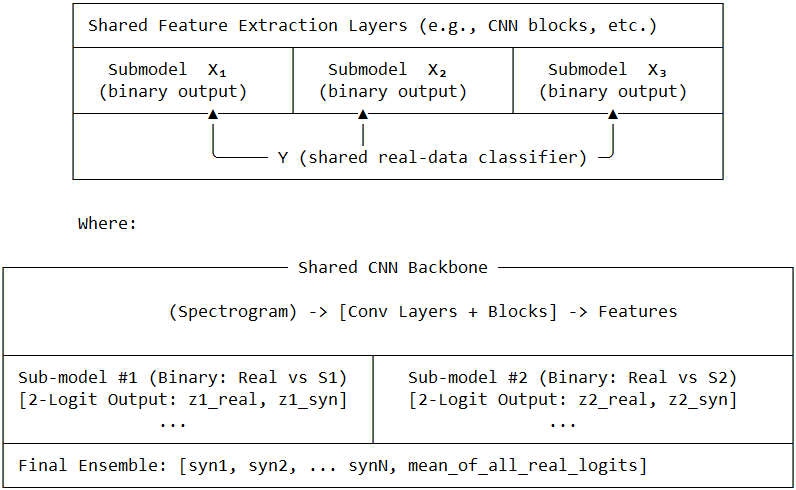
\includegraphics[width=0.7\linewidth]{figures/multihead_model_architecture.png}
    \caption{Architecture of the multi-head ensemble model. Each sub-model independently produces real and synthetic logits. The ensemble averages all real logits while keeping synthetic logits separate, creating an \(N+1\)-dimensional output where \(N\) is the number of sub-models. (S.Hibbs 2025)}
    \label{fig:multihead_architecture}
\end{figure*}

\textbf{Rationale:} Merging sub-models into one model simplifies deployment by encapsulating all components in a single module. The approach of averaging real logits and preserving synthetic logits implements the strict decision rule for authentic classification.

\textbf{Operational Integration:} Run this script once all sub-model checkpoints are available. The resulting merged model is used for inference.

\subsection{Inference Runner (\texttt{inference\_runner.py})}
This script applies the merged multi-head model to new audio data for synthetic detection.

\textbf{Functionality:}
\begin{itemize}
    \item Loads the merged model and any associated metadata.
    \item Preprocesses input audio (conversion, segmentation, mel-spectrogram transformation) using the same pipeline as for training.
    \item For each audio segment, obtains the model’s output vector, applies the decision rule (comparing synthetic logits to the averaged real logit), and determines the predicted label.
    \item For audio files that were segmented, aggregates the per-segment predictions (e.g. by averaging or majority vote) to yield an overall decision.
    \item Outputs the final result in a structured format (e.g. JSON) containing the filename, segmented predictions (with start and end times), and percentage breakdowns of class probabilities.
\end{itemize}

\textbf{Rationale:} The inference runner encapsulates the full prediction pipeline for new data, ensuring consistency with the training preprocessing. The clear output format facilitates integration with downstream systems or human review.

\textbf{Operational Integration:} Use this script by specifying the merged model checkpoint and the input file or directory to run detection on new audio data.

\section{Expected Performance and Efficiency}
Based on the design and modular nature of our system, we anticipate the following performance characteristics:
\begin{itemize}
    \item \textbf{High Detection Accuracy:} Each sub-model, trained as a binary classifier, is expected to achieve high accuracy (95--99\%) on its respective task. When merged into an ensemble, overall accuracy should reach into the high 90s.
    \item \textbf{Robustness:} Extensive augmentation and the ensemble strategy enhance generalisation, reducing both false negatives (missed fakes) and false positives (misclassifying real audio as fake).
    \item \textbf{Scalability:} The modular design allows for easy expansion by training additional sub-models for new synthetic classes without retraining existing ones.
    \item \textbf{Efficiency:} While running multiple sub-models incurs higher computational cost than a single model, the merged model is optimised to run all sub-models in a single forward pass on a GPU. Offline preprocessing (conversion, augmentation, segmentation) is parallelised to handle large datasets efficiently.
    \item \textbf{Real-Time Feasibility:} With proper batching and GPU acceleration, the system is capable of near-real-time inference on 4-second audio segments, making it suitable for applications requiring timely detection.
\end{itemize}

\begin{table}[t]
\caption{Computational Requirements for Different ResNet Backbones}
\label{tab:model_comparison}
\centering
\begin{tabular}{|l|c|c|c|c|}
\hline
\textbf{Model Type} & \textbf{Parameters (M)} & \textbf{Layers} & \textbf{Size (MB)} & \textbf{GPU Memory (GB)} \\
\hline
ResNet-18 & 11.7 & 18 & 44 & $< 2$ \\
\hline
ResNet-34 & 21.8 & 34 & 87 & $< 2$ \\
\hline
ResNet-50 & 25.6 & 50 & 102 & $< 3$ \\
\hline
ResNet-101 & 44.5 & 101 & 178 & $< 4$ \\
\hline
ResNet-152 & 60.2 & 152 & 240 & $< 5$ \\
\hline
\end{tabular}
\end{table}

While our system supports various ResNet architectures as the backbone feature extractor, resource considerations may influence the specific choice of model. Table \ref{tab:model_comparison} illustrates the parameter count, layer depth, model size, and approximate GPU memory requirements for different ResNet variants. The scalability of our approach allows practitioners to select an appropriate backbone based on the available computational resources and desired inference speed. For applications with limited computational capacity, a ResNet-18 backbone provides adequate performance while maintaining efficiency. Conversely, when prioritizing detection accuracy for high-stakes applications, the deeper ResNet-152 architecture offers enhanced feature extraction capabilities at the expense of increased computational requirements.

\begin{table}[t]
\caption{Training Performance with ResNet-152 on Various GPU Configurations}
\label{tab:training_performance}
\centering
\begin{tabular}{|l|l|c|c|c|c|}
\hline
\textbf{GPU} & \textbf{Model Type} & \textbf{Test Corpus} & \textbf{Train Corpus} & \textbf{Classes} & \textbf{Time/Epoch (H)} \\
\hline
Nvidia 3090 & ResNet-152 & 28M & 90M & 2 & 18.5 \\
\hline
Nvidia A100 $\times$ 1 & ResNet-152 & 28M & 90M & 2 & 14.0 \\
\hline
Nvidia A100 $\times$ 2 & ResNet-152 & 28M & 90M & 2 & 10.0 \\
\hline
Nvidia A100 $\times$ 4 & ResNet-152 & 28M & 90M & 2 & 5.0 \\
\hline
\end{tabular}
\end{table}

Table \ref{tab:training_performance} presents empirical training performance metrics when using the ResNet-152 backbone on various GPU configurations. The data illustrates the substantial training time reduction achieved through parallel computing. With our dataset comprising 90 million training samples and 28 million testing samples, a single Nvidia 3090 GPU requires approximately 18.5 hours per training epoch. The training time reduces nearly linearly with additional computational resources, with four Nvidia A100 GPUs completing an epoch in just 5 hours—a 73\% reduction compared to the 3090 baseline. These performance characteristics demonstrate that our system can efficiently process large-scale datasets when suitable computational infrastructure is available. For production deployments, we recommend multi-GPU training to minimize the time required for model convergence, especially when using deeper architectures like ResNet-152 that yield higher accuracy at the cost of increased computational demands.


\section{Conclusion}
This manuscript describes a sophisticated multi-head binary classification architecture for synthetic data detection, with particular application to artificially generated audio discrimination. The system integrates a parameterised feature-extraction backbone with multiple specialised classifier heads, whose probabilistic outputs are aggregated asymmetrically by averaging all real logits while preserving individual synthetic logits. This ensemble methodology improves detection sensitivity by enforcing a unanimity requirement for authentic classification, thereby reducing the risk of misclassifying synthetic content as authentic.

Our methodological contribution extends contemporary research on ensemble learning, one-versus-all taxonomic frameworks, and synthetic data detection architectures. Empirical evidence suggests that such modular, extensible designs can match or exceed the performance of monolithic models, particularly in dynamic contexts with continuously emerging synthetic techniques.

Uhmbrella Ltd. is currently applying these findings in the development of EUCLID (Enhanced Utility for Classification and Identification of Data), a comprehensive software suite designed for audio attribution and detection systems. EUCLID operationalises the multi-head classification architecture described herein, with particular emphasis on its application to copyright protection in generative AI ecosystems. One principal deployment scenario is the detection of copyrighted audio material within the tokenised outputs of generative audio AI models, a critical functionality for intellectual property protection in an era of increasingly sophisticated synthetic content generation. The system's modular architecture and extensible classification strategy make it highly suitable for rapid adaptation to novel generative techniques.

Future research will investigate further optimisation of parameter sharing among sub-models and the integration of complementary modalities (such as visual artefacts) to construct a comprehensive multimodal synthetic content detection system.

\bibliographystyle{IEEEtran}
\bibliography{references}

\section*{Figure Index}
\begin{itemize}
    \item Figure (1): Architecture of the multi-head ensemble model
\end{itemize}

\section*{Equation Index}
\begin{itemize}
    \item Equation (1): Sub-model output logits calculation
    \item Equation (2): Probability of real class from single sub-model
    \item Equation (3): Probability of synthetic class from single sub-model
    \item Equation (4): General softmax function for multi-class problems
    \item Equation (5): Ensemble's averaged real logit calculation
    \item Equation (6): Complete ensemble output vector structure
    \item Equation (7): Ensemble's probability estimation for real class
    \item Equation (8): Ensemble's probability estimation for synthetic class
    \item Equation (9): Binary cross-entropy loss function
    \item Equation (10): General cross-entropy loss for multi-class problems
    \item Equation (11): Decision rule for real vs. synthetic classification
    \item Equation (12): Product of independent real probabilities across sub-models
    \item Equation (13): Logarithmic transformation of probability product
\end{itemize}

\end{document}
